\documentclass[aspectratio=169]{beamer}
\usepackage[utf8]{inputenc}
\usepackage[spanish]{babel}
\usepackage{graphicx}
\usepackage{booktabs}
\usepackage{ragged2e}
\usepackage{minted}
\usepackage{xcolor}
\definecolor{LightGray}{gray}{0.975}
\usepackage{xcolor}
\definecolor{LightGray}{gray}{0.975}
\definecolor{links}{HTML}{2A1B81}
%\usepackage[urlcolor=blue]{hyperref}
\hypersetup{colorlinks,linkcolor=,urlcolor=blue}

\usepackage{tikz}
\usetikzlibrary{arrows,shapes}

\usepackage{algorithm}
\usepackage{algorithmic}

\usepackage{minted}
\usepackage{xcolor}
\definecolor{LightGray}{gray}{0.975}

\usepackage{listings}

%\usetheme{Warsaw}
\usefonttheme{serif} 

\title[Monitoring]{Database Administration}
\subtitle{Lecture 04: Performance Monitoring and Diagnosis.}
\author{Ciolli et al. and Grafana Labs.}
\date{\today}

\setbeamertemplate{navigation symbols}{}%remove navigation symbols

\defbeamertemplate*{footline}{shadow theme}
{%
  \leavevmode%
  \hbox{\begin{beamercolorbox}[wd=.5\paperwidth,ht=2.5ex,dp=1.125ex,leftskip=.3cm plus1fil,rightskip=.3cm]{author in head/foot}%
    \usebeamerfont{author in head/foot} Database Administration \hfill \insertshorttitle
  \end{beamercolorbox}%
  \begin{beamercolorbox}[wd=.5\paperwidth,ht=2.5ex,dp=1.125ex,leftskip=.3cm,rightskip=.3cm plus1fil]{title in head/foot}%
    \usebeamerfont{title in head/foot} \hfill \insertframenumber\,/\,\inserttotalframenumber%
  \end{beamercolorbox}}%
  \vskip0pt%
}

\AtBeginSection[]
{
     \begin{frame}<beamer>
     \frametitle{Plan}
     \tableofcontents[currentsection]
     \end{frame}
}

\newcommand{\toRight}[1]{
    \begin{FlushRight}
        {\tiny #1}
    \end{FlushRight}
} % Align to right

\begin{document}

\frame{\titlepage}

\begin{frame}{Database Administration: Performance Monitoring and Diagnosis.}
    \centering
    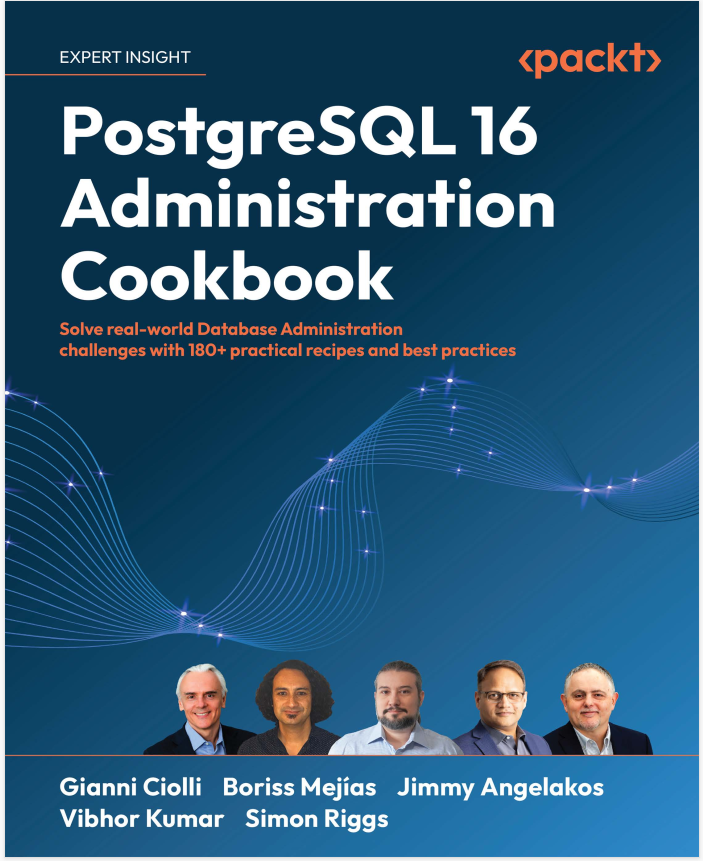
\includegraphics[width=0.35\textwidth]{figures/book_cover4}\\
    \vspace{2mm}
    {
        \scriptsize
        Content has been extracted from \textit{PostgreSQL 16 Administration Cookbook} by Ciolli, Mejías, Angelakos, Kumar \& Riggs, 2023. Visit \href{https://www.packtpub.com/en-us/product/postgresql-16-administration-cookbook-9781835468449}{packtpub.com}.
    }
\end{frame}

\section{PostgreSQL Server Logs}

\begin{frame}{Why check the server log?}
  \begin{itemize}
    \item First stop when diagnosing server issues; review it regularly.
    \item Records server messages with timestamps and PIDs, e.g.:
    \begin{itemize}
        \item \texttt{2023-09-01 19:37:41 GMT [2506-1] LOG: database system is ready to accept connections}
    \end{itemize}
  \end{itemize}
\end{frame}

\begin{frame}{Where the log can live}
  \begin{itemize}
    \item Under the data directory (one or more files).
    \item In another filesystem directory.
    \item Redirected to \texttt{syslog} (or Windows Event Log).
    \item There may be \emph{no} server log configured $\Rightarrow$ configure it!
  \end{itemize}
\end{frame}

\begin{frame}{Default locations by platform}
  \begin{itemize}
    \item Debian/Ubuntu: \texttt{/var/log/postgresql}
    \item Red Hat / RHEL / CentOS / Fedora: \texttt{/var/lib/pgsql/data/pg\_log}
    \item TPA deployments: \texttt{/var/log/postgres/postgres.log} and \texttt{syslog}
    \item Windows: Windows Event Log
  \end{itemize}
\end{frame}

\begin{frame}{File naming and rotation}
  \begin{itemize}
    \item Current file: \texttt{postgresql-\textit{MAJOR}\,-\textit{SERVER}.log} (e.g., \texttt{postgresql-14-main.log}).
    \item Older files: numeric suffix (\texttt{.1}, \texttt{.2}, \dots) --- higher number = older file.
    \item Rotation via OS \texttt{logrotate} (Debian/Ubuntu default) or PostgreSQL settings
          \texttt{log\_rotation\_age}, \texttt{log\_rotation\_size} (when using the logging collector).
  \end{itemize}
\end{frame}

\begin{frame}{Severity levels (mapping examples)}
  \centering
  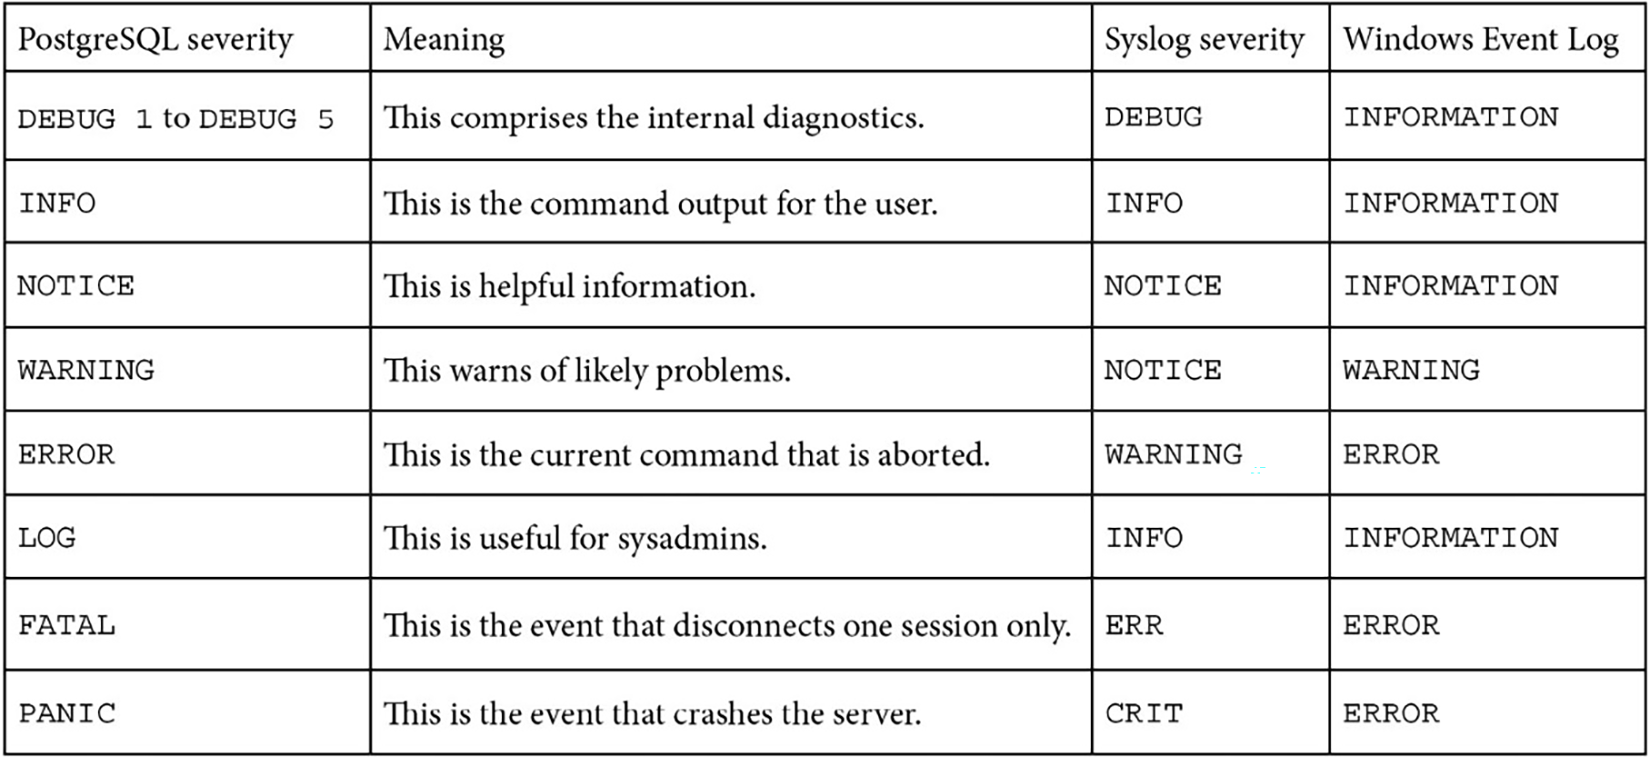
\includegraphics[width=\textwidth]{figures/postgres-severity}
  % Table illustrates PostgreSQL severities (DEBUG..PANIC) and approximate Syslog/Windows mappings.
\end{frame}

\begin{frame}{Control what gets logged}
  \begin{itemize}
    \item \textbf{log\_min\_messages}: minimum severity to record (e.g., \texttt{WARNING}, \texttt{ERROR}).
    \item \textbf{log\_error\_verbosity}: detail per event (e.g., \texttt{TERSE}, \texttt{DEFAULT}, \texttt{VERBOSE}).
    \item Other useful knobs:
      \begin{itemize}
        \item \texttt{log\_statements}, \texttt{log\_checkpoints}
        \item \texttt{log\_connections} / \texttt{log\_disconnections}
        \item \texttt{log\_lock\_waits}, \texttt{log\_verbosity}
        \item \texttt{log\_line\_prefix} (prefix fields per line)
      \end{itemize}
  \end{itemize}
\end{frame}

\begin{frame}{Where logs go \& collectors}
  \begin{itemize}
    \item \textbf{log\_destination}: \texttt{stderr}, \texttt{csvlog}, \texttt{syslog}, \texttt{eventlog (Windows)}.
    \item \textbf{logging collector}: background process that captures \texttt{stderr} output to files; reliable in failure cases.
    \item Combine with OS tools (\texttt{syslog}, \texttt{logrotate}) when appropriate.
  \end{itemize}
\end{frame}

\begin{frame}{Watch-outs \& references}
  \begin{itemize}
    \item \textbf{FATAL} and \textbf{PANIC}: unexpected in normal ops (exceptions may occur in replication scenarios).
    \item For ongoing monitoring, see practices in Chapter 8 (Monitoring and Diagnosis) and log monitoring recipes.
  \end{itemize}
\end{frame}

\section{Monitoring and Diagnosis}

\begin{frame}{Monitoring and Diagnosis}
\begin{itemize}
    \item Contains recipes for common monitoring and diagnosis tasks within PostgreSQL.
    \item Designed to answer specific, frequently encountered questions.
    \item Helps you understand and address issues while using PostgreSQL.
\end{itemize}
\end{frame}

\begin{frame}{Topics}
    \begin{itemize}
        \item Providing PostgreSQL information to monitoring tools
        \item Monitoring the PostgreSQL message log
        \item Real-time viewing using pgAdmin
        \item Checking whether a user is connected
        \item Checking whether a computer is connected
        \item Repeatedly executing a query in \texttt{psql}
    \end{itemize}
\end{frame}

\begin{frame}{Topics}
    \begin{itemize}
        \item Checking which queries are running
        \item Monitoring the progress of commands and queries
        \item Checking which queries are active or blocked
        \item Knowing who is blocking a query
        \item Killing a specific session
        \item Knowing whether anybody is using a specific table
    \end{itemize}
\end{frame}

\begin{frame}{Topics}
    \begin{itemize}
        \item Knowing when a table was last used
        \item Monitoring I/O statistics
        \item Usage of disk space by temporary data
        \item Understanding why queries slow down
        \item Analyzing the real-time performance of your queries
        \item Tracking important metrics over time
    \end{itemize}
\end{frame}

\begin{frame}{Beyond Database Monitoring}
\begin{itemize}
    \item Monitoring only the database is not enough.
    \item You must also monitor all components involved in database usage:
    \begin{itemize}
        \item Is the database host available and accepting connections?
        \item Network bandwidth usage and possible interruptions or dropped connections.
        \item RAM availability for common tasks and remaining free memory.
        \item Disk space availability and prediction of when it will run out.
    \end{itemize}
\end{itemize}
\end{frame}

\begin{frame}{Beyond Database Monitoring (cont.)}
\begin{itemize}
    \item Disk subsystem performance and capacity for additional load.
    \item CPU load and available idle cycles.
    \item Availability of dependent network services (e.g., Kerberos for authentication).
    \item Number of context switches during database operation.
    \item Historical trends for these metrics to detect changes over time.
    \item Identifying when disk usage started to change rapidly.
\end{itemize}
\end{frame}


\begin{frame}{Most Relevant Topics}
    \begin{enumerate}
        \item \textbf{Monitoring the PostgreSQL message log} – primary source for detecting errors, warnings, and server events.

        \item \textbf{Checking which queries are running} – crucial for identifying real-time performance bottlenecks.

        \item \textbf{Monitoring the progress of commands and queries} – enables tracking of long-running operations such as \texttt{VACUUM}, \texttt{ANALYZE}, and complex queries.

        \item \textbf{Identifying who is blocking a query} – essential for diagnosing lock contention and concurrency issues.

        \item \textbf{Monitoring I/O statistics} – helps detect disk-related bottlenecks and storage constraints.

        \item \textbf{Understanding why queries slow down} – supports root cause analysis of performance degradation.

        \item \textbf{Tracking important metrics over time} – lightweight monitoring of key PostgreSQL metrics and trends.
    \end{enumerate}
\end{frame}


\subsection{Monitoring the PostgreSQL Message Log}

\begin{frame}{Monitoring the PostgreSQL Message Log}
\begin{itemize}
    \item Essential in production for detecting warnings, errors, and performance trends.
    \item PostgreSQL can produce large volumes of logs daily.
    \item Use tools like \textbf{pgBadger} to:
    \begin{itemize}
        \item Summarize and analyze logs automatically.
        \item Generate reports for specific time periods.
        \item Gain insights into server activity without manual log scanning.
    \end{itemize}
\end{itemize}
\end{frame}

\begin{frame}{Getting Ready: Installation \& Rotation}
\begin{itemize}
    \item Most Linux distribution PostgreSQL packages have log file rotation enabled by default.
    \item pgBadger can be installed via your package manager:
    \begin{itemize}
        \item From community repositories.
        \item From your distribution’s own packages.
    \end{itemize}
    \item Log rotation ensures logs are manageable and archived automatically.
\end{itemize}
\end{frame}

\begin{frame}{Getting Ready: PostgreSQL Settings for pgBadger}
\begin{itemize}
    \item Configure \texttt{log\_line\_prefix} to include at least:
    \begin{itemize}
        \item \texttt{\%t} – timestamp (no milliseconds).
        \item \texttt{\%p} – process ID.
    \end{itemize}
    \item Enable parameters for richer analysis:
    \begin{itemize}
        \item \texttt{log\_checkpoints = on}
        \item \texttt{log\_connections = on}
        \item \texttt{log\_disconnections = on}
        \item \texttt{log\_lock\_waits = on}
        \item \texttt{log\_temp\_files = 0}
        \item \texttt{log\_autovacuum\_min\_duration = 0}
        \item \texttt{log\_error\_verbosity = default}
    \end{itemize}
\end{itemize}
\end{frame}

\begin{frame}{Getting Ready: Reducing Log Volume}
\begin{itemize}
    \item Use \texttt{log\_min\_duration\_statement} to limit logged queries by runtime.
    \item Example: \texttt{250ms}: only log statements longer than 250 milliseconds.
    \item Reduces unnecessary log entries while keeping slow queries visible.
    \item More details:
     \begin{itemize}
         \item PostgreSQL logging configuration: \href{https://www.postgresql.org/docs/current/runtime-config-logging.html}{PostgreSQL Docs}
         \item pgBadger configuration: \href{https://pgbadger.darold.net/documentation.html}{pgBadger Docs}
     \end{itemize}
\end{itemize}
\end{frame}

\begin{frame}{Using pgBadger with Cron}
\begin{itemize}
    \item Schedule pgBadger to run automatically via \texttt{cron}.
    \item Example: run daily at 4:00 AM to create incremental reports:
    \begin{itemize}
        \item \texttt{0 4 * * * /usr/bin/pgbadger -I -q /var/log/postgresql/postgresql.log.1 -O /var/www/pg\_reports/}
    \end{itemize}
    \item Produce:
    \begin{itemize}
        \item Daily incremental reports.
        \item Weekly summary at the end of the week.
    \end{itemize}
\end{itemize}
\end{frame}

\begin{frame}{pgBadger Reports}
\begin{itemize}
    \item Generates HTML reports with interactive JavaScript charts.
    \item Viewable directly in your browser.
    \item Can highlight:
    \begin{itemize}
        \item Top \(N\) most time-consuming queries.
        \item Performance trends and anomalies.
    \end{itemize}
\end{itemize}
\end{frame}

\begin{frame}{pgBadger Report Example}
\begin{itemize}
    \item Example of a \textbf{Time Consuming Queries} report.
    \item Shows:
    \begin{itemize}
        \item Total and average execution time.
        \item Minimum and maximum duration.
        \item Execution count.
        \item Hourly breakdown with durations.
    \end{itemize}
\end{itemize}
\end{frame}

\begin{frame}{pgBadger Report Example (Cont.)}
\begin{itemize}
    \item Interactive charts help visualize query performance trends.
\end{itemize}
\begin{center}
    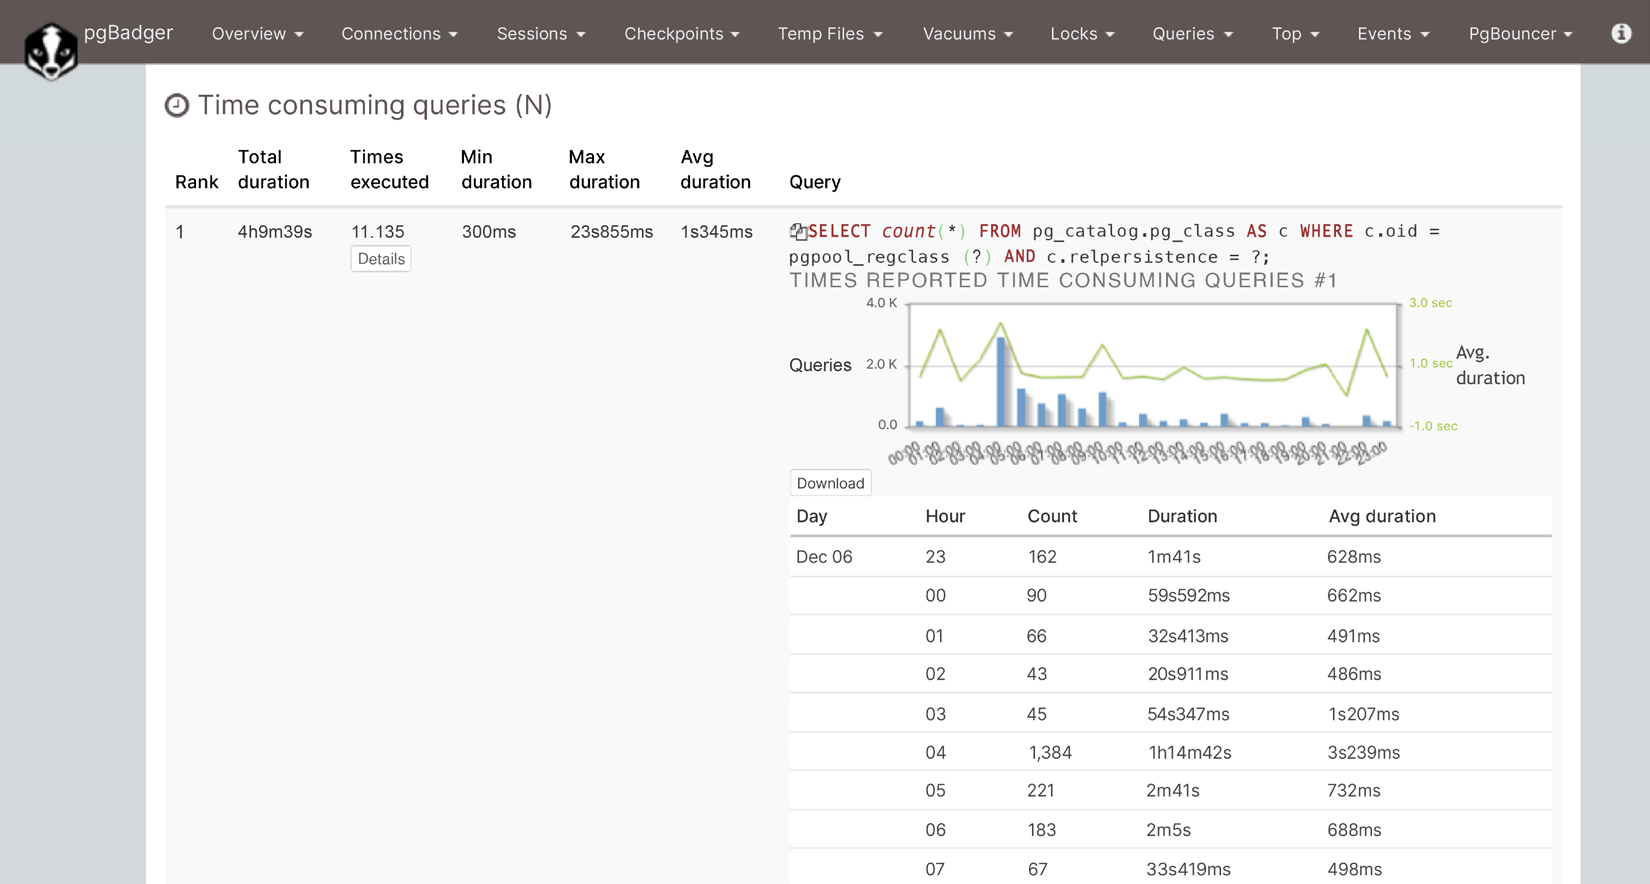
\includegraphics[width=0.9\textwidth]{figures/pgbadger}
\end{center}
\end{frame}

\subsection{Checking Which Queries Are Running}

\begin{frame}{Checking Which Queries Are Running}
\begin{itemize}
    \item Purpose: Identify currently running queries in PostgreSQL.
    \item Requirements:
    \begin{itemize}
        \item Logged in as a superuser \textbf{or} as the target database user.
        \item Ensure \texttt{track\_activities = on} (default setting).
    \end{itemize}
    \item If \texttt{track\_activities} is disabled:
    \begin{itemize}
        \item Refer to the “Updating the parameter file” recipe in Chapter 3 (Server Configuration).
    \end{itemize}
\end{itemize}
\end{frame}

\begin{frame}[fragile]{Listing All Running Queries}
\begin{itemize}
    \item To view queries currently being executed by connected users:
\begin{minted}
[tabsize=4, obeytabs, frame=lines, framesep=2mm, baselinestretch=1.2, bgcolor=LightGray, fontsize=\footnotesize, linenos]{sql}
SELECT
    datname, usename, state, backend_type, query
FROM
    pg_stat_activity;
\end{minted}
    \item \texttt{backend\_type = `client backend'} filters out PostgreSQL worker processes.
    \item Many sessions may show \texttt{state = `idle'}:
    \begin{itemize}
        \item No query running — waiting for new commands.
        \item \texttt{query} field stores the last executed statement.
    \end{itemize}
\end{itemize}
\end{frame}

\begin{frame}[fragile]{Listing Active Queries Only}
\begin{itemize}
    \item To list only active client queries:
\begin{minted}
[tabsize=4, obeytabs, frame=lines, framesep=2mm, baselinestretch=1.2, bgcolor=LightGray, fontsize=\footnotesize, linenos]{sql}
SELECT
    datname, usename, state, query
FROM
    pg_stat_activity
WHERE
    state = 'active' AND backend_type = 'client backend';
\end{minted}
    \item Focuses on currently executing statements.
    \item Helps identify ongoing workloads and potential slow queries.
\end{itemize}
\end{frame}

\begin{frame}[fragile]{How It Works: Query Activity Tracking}
\begin{itemize}
    \item With \texttt{track\_activities = on}, PostgreSQL records details for all running queries:
    \begin{itemize}
        \item Start time, state, query text, executing user, and more.
    \end{itemize}
    \item Data is accessible to users with sufficient rights via the \texttt{pg\_stat\_activity} system view.
    \item This view relies on the function:
\begin{minted}[fontsize=\scriptsize]{sql}
pg_stat_get_activity(procpid int)
\end{minted}
    \item Pass a specific \texttt{process ID} to monitor a single backend.
    \item Pass \texttt{NULL} to retrieve information for all backends.
\end{itemize}
\end{frame}

\begin{frame}[fragile]{Watching the Longest Queries}
\begin{itemize}
    \item Identify long-running queries in PostgreSQL:
\begin{minted}
[tabsize=4, obeytabs, frame=lines, framesep=2mm, baselinestretch=1.2, bgcolor=LightGray, fontsize=\footnotesize, linenos]{sql}
SELECT
    current_timestamp - query_start AS runtime,
    datname, usename, query
FROM pg_stat_activity
WHERE state = 'active'
ORDER BY 1 DESC;
\end{minted}
    \item Shows running queries ordered by execution time (longest first).
    \item Optionally add \texttt{LIMIT 10} to display only the top queries.
\end{itemize}
\end{frame}

\begin{frame}[fragile]{Filtering by Minimum Runtime}
\begin{itemize}
    \item To return only queries running for more than 1 minute:
\begin{minted}
[tabsize=4, obeytabs, frame=lines, framesep=2mm, baselinestretch=1.2, bgcolor=LightGray, fontsize=\footnotesize, linenos]{sql}
SELECT
    current_timestamp - query_start AS runtime,
    datname, usename, query
FROM pg_stat_activity
WHERE state = 'active' AND current_timestamp - query_start > '1 min'
ORDER BY 1 DESC;
\end{minted}
    \item Focuses on queries with significant execution times.
    \item Useful on busy systems to highlight potential performance issues.
\end{itemize}
\end{frame}

\subsection{Knowing Who is Blocking a Query}

\begin{frame}{Knowing Who is Blocking a Query}
\begin{itemize}
    \item Purpose: Identify the session or process causing a query to be blocked.
    \item Once a blocked query is detected, determine the blocker to resolve the issue.
    \item Requirements:
    \begin{itemize}
        \item Logged in as a \textbf{superuser} for full access to monitoring data.
    \end{itemize}
    \item Enables faster diagnosis and resolution of lock contention problems.
\end{itemize}
\end{frame}

\begin{frame}[fragile]{Identifying Blocking Sessions (Step 1)}
\begin{itemize}
    \item To find which session is blocking a query, run:
\begin{minted}
[tabsize=4, obeytabs, frame=lines, framesep=2mm,
 baselinestretch=1.2, bgcolor=LightGray,
 fontsize=\footnotesize, linenos]{sql}
SELECT datname, usename, wait_event_type, wait_event, pid,
       pg_blocking_pids(pid) AS blocked_by,
       backend_type, query
FROM pg_stat_activity
WHERE wait_event_type IS NOT NULL
  AND wait_event_type NOT IN ('Activity', 'Client');
\end{minted}
    \item Adds the \texttt{blocked\_by} column to show blocking session PIDs.
\end{itemize}
\end{frame}

\begin{frame}[fragile]{Identifying Blocking Sessions (Step 2)}
\begin{itemize}
    \item Example output:
\begin{verbatim}
-[ RECORD 1 ]---+-----------------
datname        | postgres
usename        | gianni
wait_event_type| Lock
wait_event     | relation
pid            | 19502
blocked_by     | {18142}
backend_type   | client backend
query          | select * from t;
\end{verbatim}
    \item \texttt{blocked\_by} lists one or more PIDs causing the block.
    \item PIDs are unique OS-level session identifiers.
\end{itemize}
\end{frame}

\begin{frame}{Interpreting Blocking Session Data}
\begin{itemize}
    \item \texttt{pg\_blocking\_pids(pid)} returns a list of blocking session PIDs.
    \item This query builds on the previous recipe for active or blocked queries.
    \item The \texttt{pid} column comes from the operating system and identifies each session.
    \item For more details on PIDs, see Chapter 4 (\textit{Server Control}).
\end{itemize}
\end{frame}

\begin{frame}{How It Works: Blocking Session Detection}
\begin{itemize}
    \item Uses the \texttt{pg\_blocking\_pids()} function:
    \begin{itemize}
        \item Returns an array of PIDs for all sessions blocking the given PID.
    \end{itemize}
    \item Parallel queries lock through their leader process.
    \item This behavior does not add complexity when monitoring locks.
\end{itemize}
\end{frame}

\subsection{Monitoring I/O Statistics}

\begin{frame}{Monitoring I/O Statistics}
\begin{itemize}
    \item Purpose: Assess system performance in relation to hardware resource usage.
    \item Focus: Examine I/O rates for the database and its contained objects.
    \item Requirements:
    \begin{itemize}
        \item Membership in the \texttt{pg\_monitor} role for full access to I/O statistics.
    \end{itemize}
    \item Helps identify storage bottlenecks and optimize resource usage.
\end{itemize}
\end{frame}

\begin{frame}[fragile]{Monitoring I/O Statistics with \texttt{pg\_stat\_io}}
\begin{itemize}
    \item Since PostgreSQL 16, \texttt{pg\_stat\_io} provides I/O statistics for the entire server.
    \item Includes all databases and backend types.
    \item To get running totals in bytes for each backend type:
\begin{minted}
[tabsize=4, obeytabs, frame=lines, framesep=2mm,
 baselinestretch=1.2, bgcolor=LightGray,
 fontsize=\footnotesize, linenos]{sql}
SELECT
    backend_type,
    reads * op_bytes AS bytes_read,
    writes * op_bytes AS bytes_written
FROM
    pg_stat_io;
\end{minted}
\end{itemize}
\end{frame}

\begin{frame}{PostgreSQL Maintenance Backends}
\begin{itemize}
    \item PostgreSQL uses a \textbf{process-based architecture}:
    \begin{itemize}
        \item The main server process (\texttt{postmaster} or \texttt{postgres}) spawns multiple backend processes for connections and internal tasks.
    \end{itemize}
    \item \textbf{Maintenance backends:}
    \begin{itemize}
        \item \textbf{autovacuum launcher} – Oversees autovacuum activity and schedules cleanup tasks.
        \item \textbf{autovacuum worker} – Executes vacuum and analyze operations.
        \item \textbf{background writer} – Flushes dirty buffers to disk to reduce checkpoint spikes.
        \item \textbf{checkpointer} – Writes all dirty buffers at checkpoints and updates control files.
        \item \textbf{startup} – Runs during database startup and recovery.
    \end{itemize}
\end{itemize}
\end{frame}


\begin{frame}[fragile]{Sample Output: \texttt{pg\_stat\_io}}
\begin{itemize}
    \item Example output (truncated for brevity):
\begin{verbatim}
backend_type        | bytes_read | bytes_written
--------------------+------------+---------------
autovacuum launcher |      0     |      0
client backend      |  7086080   |      0
background writer   |      0     |      0
checkpointer        |      0     | 152690688
...
(30 rows)
\end{verbatim}
    \item Shows read and write byte totals by backend type.
\end{itemize}
\end{frame}

\begin{frame}[fragile]{Per-Table I/O Statistics}
\begin{itemize}
    \item Use \texttt{pg\_statio\_user\_tables} for table-level I/O stats.
    \item Example query:
\begin{minted}
[tabsize=4, obeytabs, frame=lines, framesep=2mm,
 baselinestretch=1.2, bgcolor=LightGray,
 fontsize=\footnotesize, linenos]{sql}
WITH b AS (
    SELECT current_setting('block_size')::int AS blcksz
)
SELECT
    heap_blks_read * blcksz AS heap_read,
    heap_blks_hit  * blcksz AS heap_hit,
    idx_blks_read  * blcksz AS idx_read,
    idx_blks_hit   * blcksz AS idx_hit
FROM
    pg_statio_user_tables, b
WHERE
    relname = <table name>;
\end{minted}
\end{itemize}
\end{frame}

\begin{frame}[fragile]{Sample Output: Per-Table I/O}
\begin{itemize}
    \item Example output for table \texttt{job\_details}:
\begin{verbatim}
heap_read  | heap_hit    | idx_read | idx_hit
-----------+-------------+----------+------------
8192       | 841138176   | 8192     | 1637752832
(1 row)
\end{verbatim}
    \item Values are in bytes, calculated from block counts × block size.
\end{itemize}
\end{frame}

\begin{frame}{Interpreting PostgreSQL I/O Metrics}
\begin{itemize}
    \item \texttt{pg\_stat\_io}: server-wide I/O metrics by backend type.
    \item \texttt{pg\_statio\_user\_tables}: per-table heap and index I/O.
    \item Useful for:
    \begin{itemize}
        \item Detecting heavy I/O consumers.
        \item Balancing workloads across storage resources.
        \item Identifying caching efficiency (\texttt{hit} vs \texttt{read} ratios).
    \end{itemize}
\end{itemize}
\end{frame}


%%%%%%%%%%%%%%%%%%%%%%%%%%%%%%%%

\begin{frame}{}
    \centering
    \Huge End of Lecture 4.
\end{frame}

\section*{Takeaways}

% Tim Duncan's Top 5 Fundamental Takeaways of the Today's Class
\begin{frame}{TDT5FTOTC}
    \centering
    
\includegraphics[height=0.9\textheight]{figures/tim.png}
\end{frame}

\begin{frame}{TDT5FTOTC}
    \begin{enumerate}
        \item[5] \textbf{Log Analysis:} PostgreSQL message logs are essential for detecting issues and should be regularly analyzed with tools like \texttt{pgBadger}.\pause

        \item[4] \textbf{Query Monitoring:} Monitoring running queries in real time via \texttt{pg\_stat\_activity} helps identify and address performance bottlenecks. \pause

        \item[3] \textbf{Lock Diagnosis:} Lock contention can be diagnosed by finding blocking sessions using \texttt{pg\_blocking\_pids()}. \pause

        \item[2] \textbf{I/O Tracking:} I/O statistics from \texttt{pg\_stat\_io} and \texttt{pg\_statio\_user\_tables} reveal storage performance and caching efficiency. \pause

        \item[1] \textbf{System Health:} Full performance monitoring includes tracking CPU, RAM, disk, network, and dependent service health alongside database metrics.
        \end{enumerate}
\end{frame}

\begin{frame}{Database Administration: Performance Monitoring and Diagnosis.}
    \centering
    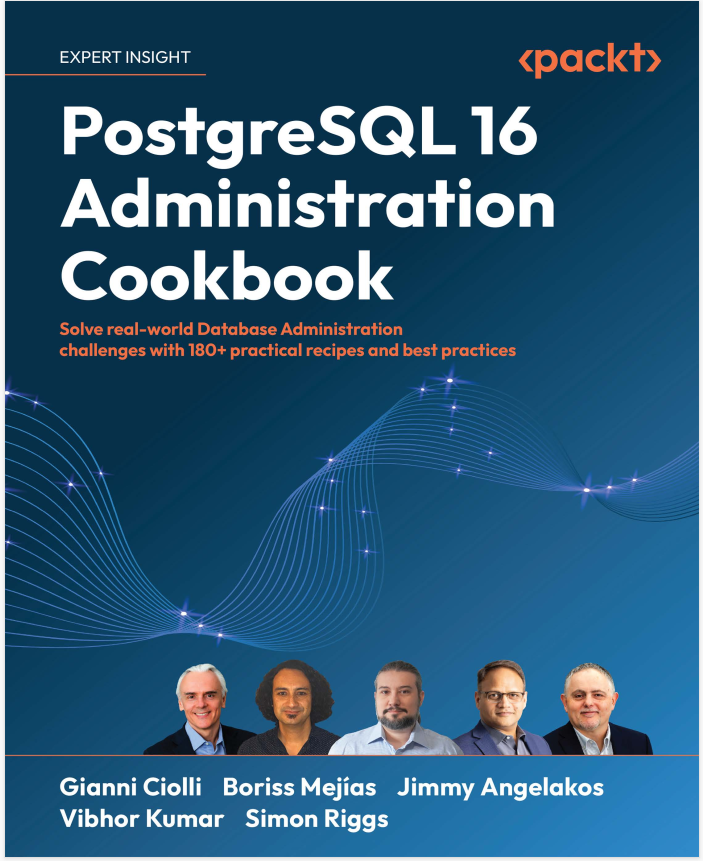
\includegraphics[width=0.35\textwidth]{figures/book_cover4}\\
    \vspace{2mm}
    {
        \scriptsize
        Content has been extracted from \textit{PostgreSQL 16 Administration Cookbook} by Ciolli, Mejías, Angelakos, Kumar \& Riggs, 2023. Visit \href{https://www.packtpub.com/en-us/product/postgresql-16-administration-cookbook-9781835468449}{packtpub.com}.
    }
\end{frame}

\end{document}
